\documentclass[12pt]{article}
\usepackage{apacite,rotating,array,booktabs,ctable,graphicx,tabularx,amsfonts, amsmath, amsthm,url,multirow,verbatim}
\usepackage[top=1in,right=1in,left=1in,bottom=1in]{geometry}
\usepackage[sc]{mathpazo}
\linespread{1.05}         % Palatino needs more leading (space between lines)
\usepackage[T1]{fontenc}
\usepackage{setspace}
\usepackage{lineno}
\linenumbers



\newcommand{\putbib}[1]{
\bibliographystyle{apacite}
\bibliography{./#1}
}	
\title{Analysis of a scale hierarchy OR Model Selection by Testing Conjoint Checks}
\date{}

\begin{document}
\maketitle
\onehalfspacing
\section{Background}
This paper discusses the application of the `conjoint checks' (CC)methodology described in \citeA{domingue2013} to the Tenable Assessment (TA) model selection framework \citeNP{torres2012}. The CC method offers a more generally applicable alternative for identifying the correct generating model of a dataset that the \textsc{bic}-based comparison originally used by \citeA{torres2012}.

The TA model selection framework \citeNP{torres2012} arranges a set of latent variable models, including latent class models (\textsc{lca}; Lazarasfeld \& Henry, 1968), ordered latent class models (\textsc{olca}; Croon, 1990), latent class Rasch models (\textsc{lcr}; Formann, 1985) and Rasch models (\textsc{rsh}; Rasch, 1960), according to their assumed latent structure such that progressively more stringent monotonicity and scale assumptions are placed on the latent variable. 

\begin{figure}
\centering
\caption{Tenable Assessment Model Selection Framework} \label{orig}
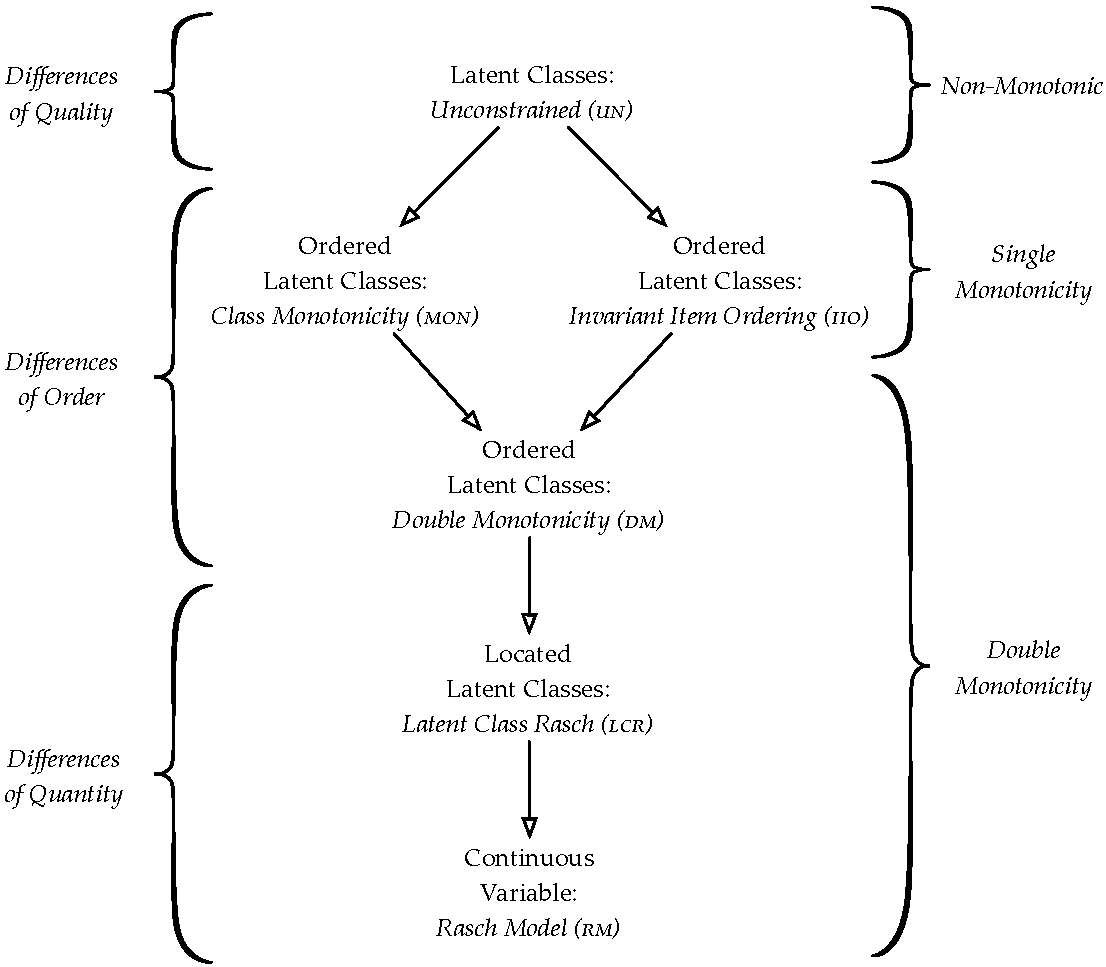
\includegraphics[width=\textwidth]{./figs/TAmodelframework.pdf}
\end{figure}

Accordingly, these models conform a hierarchy where different levels support different kinds of inference:

\begin{itemize}
	\item \textsc{lca} allows qualitative distinctions between groups.
	\item \textsc{olca} support ordinal inference about persons (when class monotonicity is enforced), items (when invariant item ordering is imposed), or both items and persons (when double monotonicity is applied).
	\item \textsc{lcr} and \textsc{rsh} entail inferences about quantitative differences.
\end{itemize}

The jump from qualitative groups to ordinal levels, and from ordinal levels to quantitative differences comes at the additional cost of considerably more stringent assumptions. 

% to make tenable inference using these models, the observed data should be consistent 

For data to adequately fit with the latter models, it must be consistent with the the axioms of single (in the case of ordinal models) and double cancellation as described by the theory of additive conjoint measurement (\textsc{adm}; \citeNP{luce1964})\footnote{The higher-order axioms of solvability and the Archimedean condition are typically impossible to verify in practice.}.

The methodology developed by \citeA{domingue2013} and implemented in \citeA{conjointchecks} describes a procedure for checking the consistency of such axioms, and presents a more flexible alternative to the \textsc{bic} based model selection criteria originally used by \citeA{torres2012}, supporting the use of the tenable assessment model selection framework on datasets with larger number of items.

\subsection{Examining Cancellation Axioms}

The Tenable Assessment framework \citeNP{torres2012} leads to several natural hypotheses regarding potential violations to the \textsc{acm} cancellation axioms:

\begin{enumerate}
\item The UN model, since it can be fit to purely nominal data, should yield the most violations.
\item At least superficially, there is no reason that there should be substantial differences in the number of detected violations between the MON and IIO models since they each support only a single version of the single cancellation axiom.
\item The DM model supports both version of single cancellation but is not necessarily consistent with single cancellation. Hence, it should produce fewer violations than the IIO and MON models but more than the LCR and RSH models.
\item The LCR and RSH models should produce the fewest number of violations given that they are both consistent with single and double cancellation.
\end{enumerate}
Note that from the point-of-view of the hierarchy given in Figure \ref{orig}, there should be no difference in the findings with respect to the axioms between the LCR and RSH models. However, there is clearly an important difference between the two since the former allows for only a discrete number of classes while the latter allows for a continuum of scores. 

If these hypotheses hold, then the methodology from \citeA{domingue2013} would provide a fairly simple and convenient criteria to conduct a model selection procedure under the Tenable Assessment Framework. However, the results discussed in this paper do not seem to fully meet the original expectations, prompting additional investigation. For example, it will be seen that the MON and IIO models produce quite different numbers of axiom violations and this leads us to ask what it is about these models that causes this difference. Alternatively, a failure to find evidence that supports the hypotheses related to double cancellation leads us to argue that checking for double cancellation is probably an intractable problem given the `messy nature of the data in question.

\section{Models}
describe the models in the scale hierarchy. 

 
\section{Results}

N different data sets were then simulated using each of the six different generating models. Each of the datasets was then checked. Results are shown in Figure \ref{boxplots}. For violations detected in both randomly formed 3-matrices as well as adjacent 3-matrices, the algorithm clearly distinguishes between the UNC and MON models on one hand and the IIO, DM, LCR, and RSH models on the other. The fact that there is a substantial difference between the IIO and the MON models is surprising given that these models are formally symmetric. It appears that the checks are sensitive to poorly ordered columns but insensitive to ambiguities in row ordering, but this is actually too simple an explanation. This issue is explored at length in Section \ref{iio_mon}.

That the algorithm, which simultaneously checks for both forms of single cancellation as well as double cancellation, can not distinguish between the IIO, DM, LCR, and RSH models is surprising given that IIO and DM do not support double cancellation in general while LCR and RSH do. The checks seem relatively insensitive to violations of double cancellation. Section \ref{sc_dc} further explores why the checks can not detect violations of double cancellation and also demonstrates that checks for double cancellation are quite challenging given the ``messiness'' of real-world data and add little to checking simply for both forms of single cancellation.\footnote{It may in fact be the case that checking double cancellation in the presence of measurement error is just as challenging as checking the other higher-order axioms!} 
% Finally, Section \ref{distort} probes the problems that may arise if data generated via the LCR is mistakenly fitted with the RSH.

\begin{figure}
\centering
\caption{Boxplots showing distribution of violation means (for 3-matrices from randomly chosen and adjacent rows and columns) for the different models} \label{boxplots}
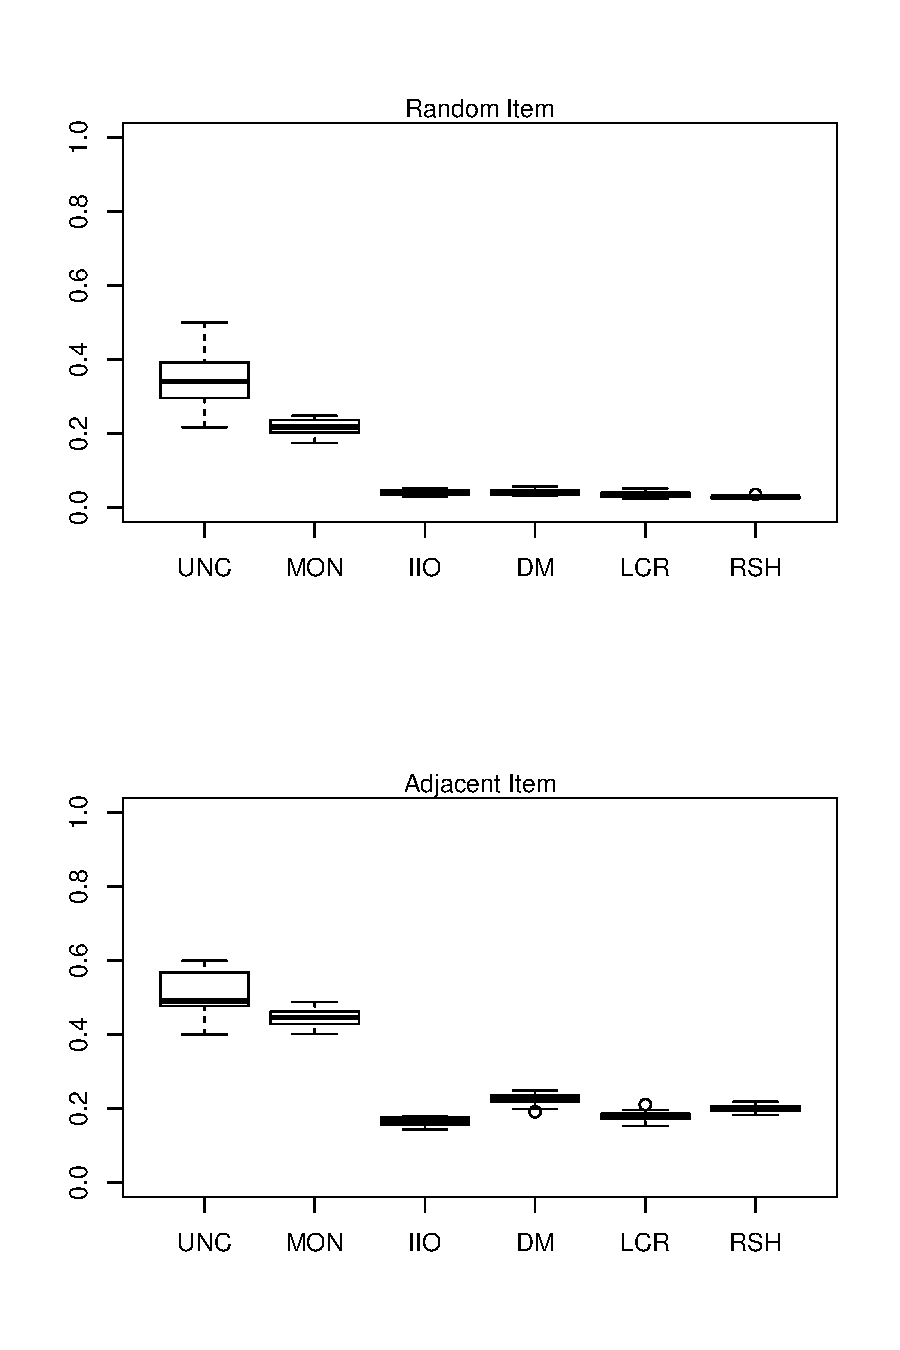
\includegraphics[height=\textheight]{./figs/boxplots}
\end{figure}

\subsection{IIO versus MON} \label{iio_mon}
Recall that the IIO model allows for clear ordering of columns while the MON model {\em should} allow for clear ordering of rows. Figure \ref{boxplots_single} compares violation proportions for checks testing only row or column versions of single cancellation in adjacently formed 3-matrcies. The top panel demonstrates that the checks are relatively insensitive to violations associated with column ordering\footnote{there is something about this result that i'm not totally comfortable with and it has to do with the fact that with the mon models, the item parameters should be `singular' and yet i'm convinced that they're being accurately estimated and this leads to the low violations. what if we looked at fit statistics or SEs for the item parameters here?
ONE WAY OF TESTING THIS WOULD BE TO VARY THE DIFFERENCES BETWEEN THE DIFFICULTIES OF THE COLUMNS. TIGHTER ITEMS, IN THAT THEIR DIFFICULTIES ARE CLOSER, SHOULD LEAD TO MORE ERRORS (AT LEAST FOR IIO). FOR MON, NEED TO EXPERIMENT WITH HOW BAD THE ITEM VIOLATIONS ARE.}, but it is reassuring to note that fewer violations are detected with data generated from the IIO model. The bottom panel shows that the MON model generates large numbers of row violations. Note that it is suprising that the IIO model does not since individuals can not be consistently ordered with this model.  Given that MON maintains person ordering, in contrast to IIO, the opposite is to be expected. The next several sections are an investigation into why we observe so many more MON violations. 

\begin{figure}
\centering
\caption{Boxplots showing distribution of violation means for  separate checks of single cancellation} \label{boxplots_single}
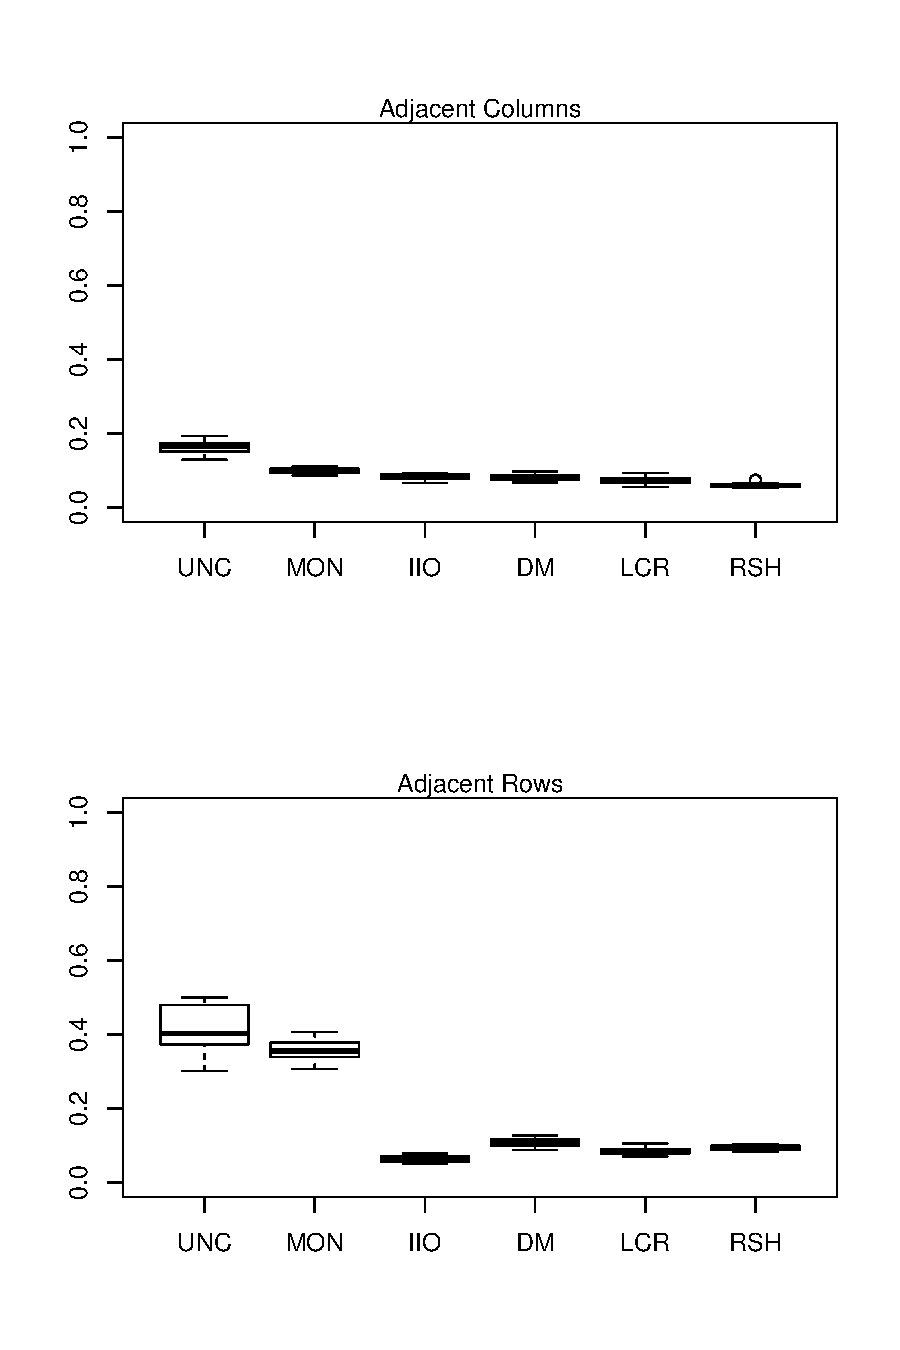
\includegraphics[height=\textheight]{./figs/boxplots_single}
\end{figure}

\subsubsection{What is the difference between person and item violations?}
One potential theory for why row violations are so readily detected is that row ``estimates'' come with two sources of error:
\begin{enumerate}
\item Error in estimates of individual abilities.
\item Error in aggregating rows of common abilities.
\end{enumerate}
In contrast, column orderings only have error due to the error in individual item parameters (which are also more precisely estimated than individual person parameters). Table \ref{inc.precise} is a first attempt to make sense of this issue. A simulation involving responses (generated via the Rasch model) from  5000 individuals to a varying number of items was considered. The first form of the test involved only 45 items. With that form, we are generating more violations involving rows (11.6\%) than columns (7.3\%). When ability estimates are more accurate, estimates are based on responses to 450 items, there is little difference between the violations for the version of single cancellation involving rows and the version involving columns. What is curious is that there has been an uptick in the overall percentage of violations for both forms of single cancellation with this increased precision of ability estimates.\footnote{One reason for this could be the row aggregation issue discussed below. Another could be the ``mesh'' issue discussed in my dissertation.}
\ctable[
pos=ht,
caption=Increasing precision of ability estimates,
label=inc.precise,
]{lcc}{
\tnote[a]{45 items.}
\tnote[b]{450 items.}
}{
\toprule
&Rows&Columns \\ \midrule
Normal Precision\tmark[a]&11.6\% & 7.3\% \\
Increased Precision\tmark[b]&19\% & 19.2\% \\
\bottomrule
}

\subsubsection{Effect of row aggregation on violations?} \label{noisy_rows}
Consider a series of simulations based on 5000 respondents whose abilities are drawn from a normal distribution and three forms of a test: short, medium, and long. The short form, shown on the top of Figure \ref{noise}, consists of 20 items. Figure \ref{noise} displays the true score SD for all true scores whose simulated response strings yield a given sum score. For the short form, each sum score contains a set of indivuals the SD of whose true scores is fairly consistently equal to {\em or greater than} the SD of all the true scores. This is a different way of looking at measurement error. From this perspective, the sorting done by the test of the respondees into different ability groups is no greater than we would expect than if the respondees were just sorted randomly. The medium length test form, 50 items, has a true score SD for each sum score that is typically around 1/3 of the overall true score SD. The long form, 500 items, is too long to be practical for most applications but is considered as an example. For this form, the true score SD for each sum score is around 20\% of the overall true score SD.

\begin{figure}
\centering
\caption{SD in true scores as a function of observed sum scores.} \label{noise}
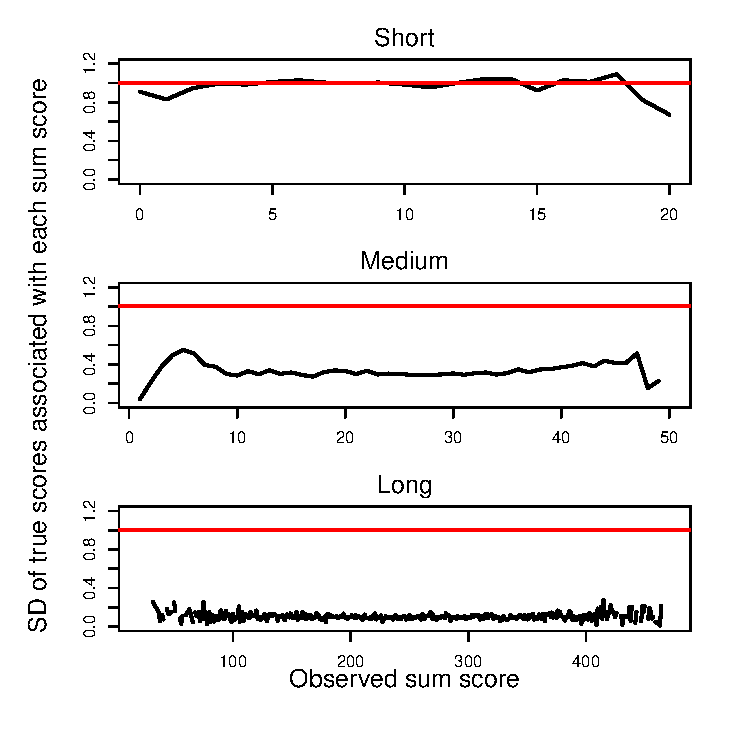
\includegraphics[width=\textwidth]{./figs/noise}
\end{figure}

\subsection{Reconsidering double cancellation} \label{sc_dc} 
As described in \citeA{domingue2013}, checking for double cancellation is challenging due to the lack of order along the minor diagonals. Evidence presented in the below sections demonstrate that, in fact, there tends to be little difference between the checks with double cancellation, as implemented in \citeA{conjointchecks}, and a version that only requires both forms of single cancellation. To illustrate this point, data from \citeA<Table 2>{perline1979} is used.

\subsubsection{No advantage to double cancellation}
Figure \ref{single_example} compares mean violation rates for the adjacent and random checks when single and double cancellation are checked (denoted double) as opposed to only single cancellation (denoted single). For the random checks, there are essentially no differences. For the adjacent checks, there are small differences for items 3, 5, and 7. For these three, the addition of the double cancellation check adds a small amount of stringency. This is perhaps rather surprising. The next section is an attempt to demonstrate why this is happening.


\begin{figure}
\centering
\caption{Comparison of violation means for single and single+double cancellation checks.} \label{single_example}
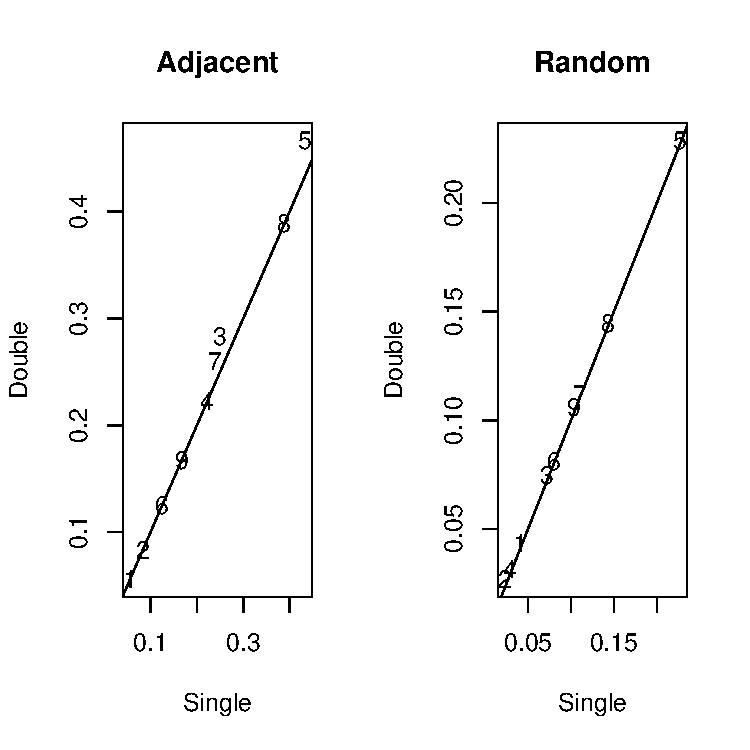
\includegraphics[width=\textwidth]{./figs/single_example}
\end{figure}

\subsubsection{The difficulty of checking for double cancellation}
To understand why double cancellation is such a fickle issue with empirical data, it will help to demonstrate via a few empirical examples. Let us begin with rows 3 through 5 of the \citeA{perline1979} data and items 2, 4, and 9. The empirical proportions are:
\[
\begin{array}{ccc}
0.15& 0.39& 0.67 \\
0.24 &0.40 &0.70 \\
 0.33& 0.51& 0.78 
\end{array}.
\]
This 3-matrix was chosen since it is seemingly (in terms of observed data, not true values) in compliance with one form of double cancellation. Focus on the $(1,3)$ element. Given the fact that $0.24<0.39$ and $0.51<0.70$, it should be (and is) the case that $0.33<0.67$. Let us monitor the nature of the checks as iterations of the Markov chain are accumulated. The basic fact is that the addition of double cancellation here is just not especially stringent. As an example, here are the updated values after the first 1000 iterations of the chain:
\[
\begin{array}{ccc}
0.14 &0.28& 0.62 \\
 0.23& 0.42& 0.65 \\
 0.31& 0.53& 0.86
\end{array}.
\]
In terms of the limits that make up the jumping distribution in the ``woven''\footnote{I'm introducing this term to deal with the fact that these chains are being updated simultaneously.} Metropolis-Hastings algorithm, the upper-right cell needs to be bigger than 0.28 because of single cancellation and, given that the precedent of double cancellation seems to hold, larger than 0.31. This difference is very slight. Checking for only single cancellation is effectively no different.

If we now look at rows 4 through 6 and columns 4 through 6, we observe a much messier scenario:
\[
\begin{array}{ccc}
 0.40& 0.52& 0.51 \\
 0.51& 0.73& 0.68 \\
 0.58& 0.95& 0.91
\end{array}.
\]
Here we have an example where a consequent of double cancellation regarding the order of the $(1,3)$ and $(3,1)$ cells is unneccessary since there is no consistent ordering regarding the pairs $(1,2),(2,1)$ and $(2,3), (3,2)$. One final example will round out the demonstration. Consider
\[
\begin{array}{ccc}
0.064 &0.23 &0.51 \\
0.180 &0.33 &0.61 \\
0.524& 0.51& 0.64
\end{array}.
\]
One form of single cancellation seems violated here. However, the violation is so slight that checking for double cancellation on top of single cancellation yields no additional information. 

For the data examined here, there are only 5 cases where 3-matrices formed from adjacent cells have empirical proporotions of correct responses that correspond to violations of double cancellation and none of these 3-matrices are violations in the sense described in \citeA{domingue2013}. An alternative way of understanding what is going on might be to compare double cancellation within simulated Rasch data. Let $S_1$ be the truth value of the statement $\theta_{2,1}>\theta_{1,2}$ and $S_2$ the truth value of the statement $\theta_{3,2}>\theta_{2,3}$. These are the statements that are involved in both forms of the interesting statement of double cancellation. Let $S_3$ be the truth value of $\theta_{3,1}>\theta_{1,3}$. Table \ref{dc.sim} tabulates these truth values from a DESCRIBE SIMULATION. Bold numbers in the table indicate violations. Note that there are no violations with the true probabilities from the Rasch model. This is to be expected given that the Rasch model is known to uphold the axioms of additive conjoint measurement. However, with the observed proportions, we observe violations in quite a large number of cases (proportionally) compared to other possibilities. The punchline is that double cancellation is ``violated'' with observed proportions even when the underlying probabilities are consistent with the axioms of ACM. Why is this? RELATE IT BACK TO SECTION \ref{noisy_rows}.


\ctable[
pos=ht,
caption=Double Cancellation with simulated Rasch data,
label=dc.sim,
]{lcccc}{
}{
\toprule
&&&\multicolumn{2}{c}{$S_3$} \\ \cmidrule{4-5}
&$S_1$&$S_2$&TRUE&FALSE \\ \midrule                       
\multirow{4}*{True Probabilities}&TRUE&TRUE&      5&     {\bf 0} \\
&TRUE&FALSE      &       9   &12 \\
&FALSE&TRUE&      8&    8\\
&FALSE&FALSE&       {\bf 0}&    7 \\ \midrule
\multirow{4}*{Observed Proportions}&TRUE&TRUE&      9&    {\bf 9} \\
&TRUE&FALSE&       7&    5 \\
&FALSE&TRUE &      8&    3 \\
&FALSE&FALSE   &    {\bf 6}&    2 \\ \bottomrule
}



Perhaps make point that it is the unevenness of the items and ability levels that leads to the disorder on the minor diagonal.



\section{Discussion}

\putbib{conjoint}

\end{document}
